\documentclass[uplatex,dvipdfmx,a4j,12pt]{jsarticle}

\usepackage[utf8]{inputenc}
\usepackage{graphicx}
\usepackage{amsmath}
\usepackage{comment}
\usepackage{color}
\usepackage{url}
\usepackage{siunitx}
\usepackage[version=4]{mhchem}
\usepackage{paralist}
\usepackage{longtable}
\usepackage{multirow}
\usepackage[dvipdfmx]{hyperref}
\usepackage{pxjahyper}

\usepackage{enumitem}
\setlist[description]{parsep=5pt}
\setlist[enumerate]{parsep=5pt}

% 半角文字のパーセント、より右側は、コメントとして扱われます。

% タイトルページの内容をここで記述します。
%
\title{
  物理学実験 II\\    % \\ は、強制的に改行するコマンドです。
  課題0 「Overleaf 上で \LaTeX を使った \\レポート作成練習」
  }
\author{
  氏名: \\
  実験者番号: % 学籍番号ではありません。
  }
\date{2025年 x月 x日}  % 提出日を記入して下さい


% ここから本文が始まります。
\begin{document}

% 上で設定したタイトルページの情報は、\maketitle があって始めて、コンパイル後に表示されます。
\maketitle


% 概要は論文・レポート全体を一つの段落にまとめたものです。
% 物理の分野では、概要では段落分けをしません。
%
\begin{abstract}
    \LaTeX を使って文章を作成する練習を行った。
    % この概要欄の文章を自分が行ったことについてまとめて下さい。
\end{abstract}


\section{数式の練習}

% 以下の文章と式を、自分の好きな数式の説明と数式に書き換えて下さい。

特殊相対性理論における、エネルギー($E$)と質量($m$)の等価性として$E=mc^2$が挙げられる。
ここで、$c$は真空中の光速度である。
これは静止している粒子に対する式であり、運動量$p$の粒子に対しては、以下の式~\eqref{eq:relative}となる。 
\begin{equation}
%
    E^2 = (m c^2)^2 + (pc)^4
    \label{eq:relative}
\end{equation}

% subsectionの部分は、提出時には消すこと。
\subsection{数式の引用の仕方について}
\LaTeX では、別行建ての数式を書く場合には、以下のようになっている

\begin{verbatim} % LaTeXのコマンドをそのまま表示させるための環境
 \begin{equation}
    E^2 = (m c^2)^2 + (pc)^4
    \label{eq:relative}
 \end{equation}
\end{verbatim}
数式には、自動的に通し番号が振られる。
ここで、\verb|\label{eq:relative}|は、数式を引用するために使うラベルを指定するコマンドで、\verb|{}|の中にある文字列(今の場合は、)がその数式のラベルである。

数式を引用するためのコマンドが、\verb|\eqref{}|である。\verb|{}|の中でラベルを指定すると、対応する数式に振られた番号が自動的に使われる。

\section{表の練習}

%以下の文章と表を、適当な表に置き換えて、その表を引用する文章に換えて下さい。

表~\ref{table:recipe}に例を示す。
この表は、LaTeXを用いたレポートの書き方の例としてこのテンプレートにある「我が家のオーブンを用いた場合のマカロンの最適な焼き方」からのコピーである。

\begin{table}[t]
    \centering
    \caption{マカロンの材料。作成の際に使う順番に並べてある。乾燥卵白以外はスーパーの製菓コーナーでよく見かけるものである。}
    \begin{tabular}{lr}
        材料              & 質量 \\
        \hline
        グラニュー糖      & 17g \\
        乾燥卵白         & 3g \\
        卵白             & 50g \\
        アーモンドプードル & 50g \\
        純粉糖 & 90g \\
        \hline
    \end{tabular}
    \label{table:recipe}
\end{table}

\section{図の練習}

図~\ref{fig:fig06}に例を示す。この図は、表のところと同じ文章からのコピーである。

\begin{figure}[b]
    \centering
    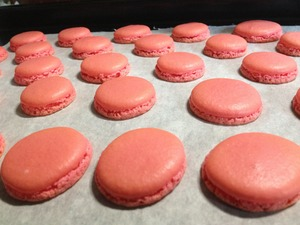
\includegraphics[width=0.3\linewidth]{fig06.jpg}
    \caption{最終的な焼き時間として採用したマカロンの焼き上がりの写真。五回目の焼き方で焼いたものである。}
    \label{fig:fig06}
\end{figure}


\end{document}
